\chapter{Graphical Models}

\begin{multicols}{2}
\noindent Bayesian networks is a probabistic graphical model that represents a set of random variables and their conditional dependencies via directed acyclic graph, where:
\begin{itemize}
    \item Nodes are the random variables
    \item Edges are conditional probabilities
\end{itemize}

\noindent Property 1: any joint probability of a directed acyclic graph can be factorized as a product of conditional distributions:
$$P(X_1,\ldots,X_n) = \prod_i P(X_i|\text{parent}(X_i))$$ \\

\section{Backgroun: Independence}

\noindent $X$ and $Y$ are independent if:
$$P(X,Y) = P(X)P(Y)$$
\noindent $X$ and $Y$ are conditionally independent given $Z$ if:
$$P(X,Y|Z) = P(X|Z) P(Y|Z)$$
$$P(X|Y,Z) = P(X|Z)$$

\section{Property 2 of Bayesian Network}

\noindent Property 2: conditional independence tells us the situation when 2 variables in a Bayesian network are conditionally independent given another variable. There are three common cases.

\subsection{Case 1: Head-to-tail Connection}
\begin{center}
\begin{tikzpicture}[
roundnode/.style={circle, draw=black, thin},
]
%Nodes
\node[roundnode](X){X};
\node[roundnode](Y)[right=of X]{Y};
\node[roundnode](Z)[right=of Y]{Z};
 
%Lines
\draw[->] (X.east) -- (Y.west);
\draw[->] (Y.east) -- (Z.west);
\end{tikzpicture}
\end{center}

\noindent Three events may be connected serially. We see here that $X$ and $Z$ are independent given $Y$ : Knowing $Y$ tells $Z$ everything; knowing the state of $X$ does not add any extra knowledge for $Z$; we write $P(Z|Y,X) = P(Z|Y)$. We say that $Y$ blocks the path from $X$ to $Z$, or in other words, it separates them in the sense that if $Y$ is removed, there is no path between $Z$ to $Z$. In this case, the join probability and be written as:
\begin{equation*}
\begin{split}
    P(X,Y,Z) &= P(X) P(Y|X) P(Z|Y,X)\\
    &= P(X) P(Y|X) P(Z|Y)
\end{split}
\end{equation*}

\noindent If we do not know the state of $X$, then
$$P(Y) = P(Y|X) + P(Y|\sim X)$$
$$P(Z) = P(Z|Y) + P(Z|\sim Y)$$

\noindent If we know the state of $X$, we can say that $Z$ is:
$$P(Z|X) = P(Z|Y)P(Y|X)+P(Z|\sim Y)P(\sim Y|X)$$

\noindent If we know the state of $Z$, we can say that $X$ is:
$$P(X|Z) = \frac{P(Z|X)P(X)}{P(Z)}$$

\subsection{Case 2: Tail-to-tail Connection}

\begin{center}
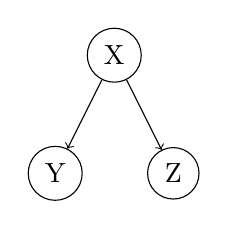
\begin{tikzpicture}[
roundnode/.style={circle, draw=black, thin},
]
%Nodes
\node[roundnode,draw](X){X}
    child {node[roundnode,draw](Y){Y} edge from parent[->]}
    child {node[roundnode,draw](Z){Z} edge from parent[->]}
;
\end{tikzpicture}
\end{center}

\noindent The joint probability is written as:
$$P(X,Y,Z) = P(X) P(Y|X) P(Z|X)$$

\noindent Normally, $Y$ and $Z$ are dependent through $X$; given $X$, $Y$ and $Z$ become independent. $X$ blocks the path between $Y$ and $Z$:
\begin{equation*}
\begin{split}
    P(Y,Z|X) &= \frac{P(X,Y,Z)}{P(X)} \\
    &= \frac{P(X) P(Y|X) P(Z|X)}{P(X)} \\
    &= P(Y|X) P(Z|X)
\end{split}
\end{equation*}

\noindent Knowing $Z$, we can infer that:
\begin{equation*}
\begin{split}
    P(X|Z) &= \frac{P(Z|X)P(X)}{P(Z)} \\
    &= \frac{P(Z|X)P(X)}{\sum_X P(Z,X)} \\
    &= \frac{P(Z|X)P(X)}{P(Z|X)P(X) +P(Z|\sim X)P(\sim X) }
\end{split}
\end{equation*}

\noindent Not knowing $X$ and knowing $Y$, we can infer $X$ which can be used to infer $Z$:
\begin{equation*}
\begin{split}
    P(Z|Y) &= \sum_X P(Z,X|Y)\\
    &= P(Z|X)P(X|Y) + P(Z|\sim X)P(\sim X|Y) \\
    &= P(Z|X) \frac{P(Y|X)P(X)}{P(Y)} + \\
    & \ \ \ \ P(Z|\sim X) \frac{P(Y| \sim X) P(\sim X)}{P(Y)}
\end{split}
\end{equation*}

\subsection{Case 3: Head-to-head Connection}
\begin{center}
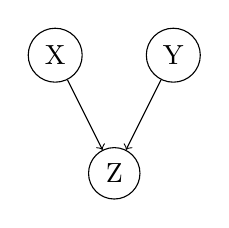
\begin{tikzpicture}[
roundnode/.style={circle, draw=black, thin},
]
%Nodes
\node[roundnode,draw](Z){Z} [grow'=up]
    child {node[roundnode,draw](X){X} edge from parent[<-]}
    child {node[roundnode,draw](Y){Y} edge from parent[<-]}
;
\end{tikzpicture}
\end{center}

\noindent The joint density is written as:
$$P(X,Y,Z) = P(X) P(Y) P(Z|X,Y)$$

\noindent $X$ and $Y$ are independent:
$$P(X,Y)=P(X)P(Y)$$

\noindent but $X$ and $Y$ become dependent when $Z$ is known. When Z (or any of its descendants) is observed, they are not blocked, separated, nor are independent. The path between X and Y is blocked, or they are separated, when Z is \textit{not} observed.

\noindent Not knowing anything else, the probability of $Z$ is:
\begin{equation*}
\begin{split}
    P(Z) &= \sum_{X,Y} P(Z,X,Y) \\
    &= P(Z|X,Y) P(X,Y) + \\
    &\ \ \ \ P(Z|X,\sim Y) P(X,\sim Y) + \\
    &\ \ \ \ P(Z|\sim X,Y) P(\sim X,Y) + \\
    &\ \ \ \ P(Z|\sim X,\sim Y) P(\sim X,\sim Y) \\
    &= P(Z|X,Y) P(X) P(Y) + \\
    &\ \ \ \ P(Z|X,\sim Y) P(X) P(\sim Y) + \\
    &\ \ \ \ P(Z|\sim X,Y) P(\sim X) P(Y) + \\
    &\ \ \ \ P(Z|\sim X,\sim Y) P(\sim X) P(\sim Y)
\end{split}
\end{equation*}
 
\noindent If we know $X$:
\begin{equation*}
\begin{split}
    P(Z|X) &= \sum_Y P(Z,Y|X)\\
    &= P(Z|Y,X) P(Y|X) + P(Z|\sim Y,X) P(\sim Y|X) \\
    &= P(Z|Y,X) P(Y) + P(Z|\sim Y,X) P(\sim Y) 
\end{split}
\end{equation*}

\noindent We also can calculate:
$$P(X|Z) = \frac{P(Z|X)P(X)}{P(Z)}$$
$$P(X|Y,Z) = \frac{P(Z|X,Y) P(X|Y)}{P(Z|X)}$$

\end{multicols}
